%!TEX root = ../INTO-CPS-Manifesto.tex

\section{The INTO-CPS Tool Chain}\label{sec:toolchain}

\fbox{Christian K\"{o}nig with support from Etienne Brosse}

\fbox{make sure that this section fits to the other sections, incl. references}

\fbox{indicate maturity of the different tool features, in particular wrt. the new ones}

This section discusses the interconnectivity of the different tools, and how the tools fit into the workflows and tasks that are covered by INTO-CPS. In particular, this section focuses on the features that were added during the INTO-CPS project, and in the framework of the INTO-CPS association. This section does \textit{not} describe all the tools in detail (here, the reader is referred to the different manuals, and to the User Manual (ref to the INTO-CPS tool manual).

An overview of the different tools that form the tool-chain of the INTO-CPS association, is given in Figure \ref{fig:tool-chain}.

[text on the overall tool-chain, refer to workflows, probably from previous section]

\begin{figure}[!ht]
	\centering
		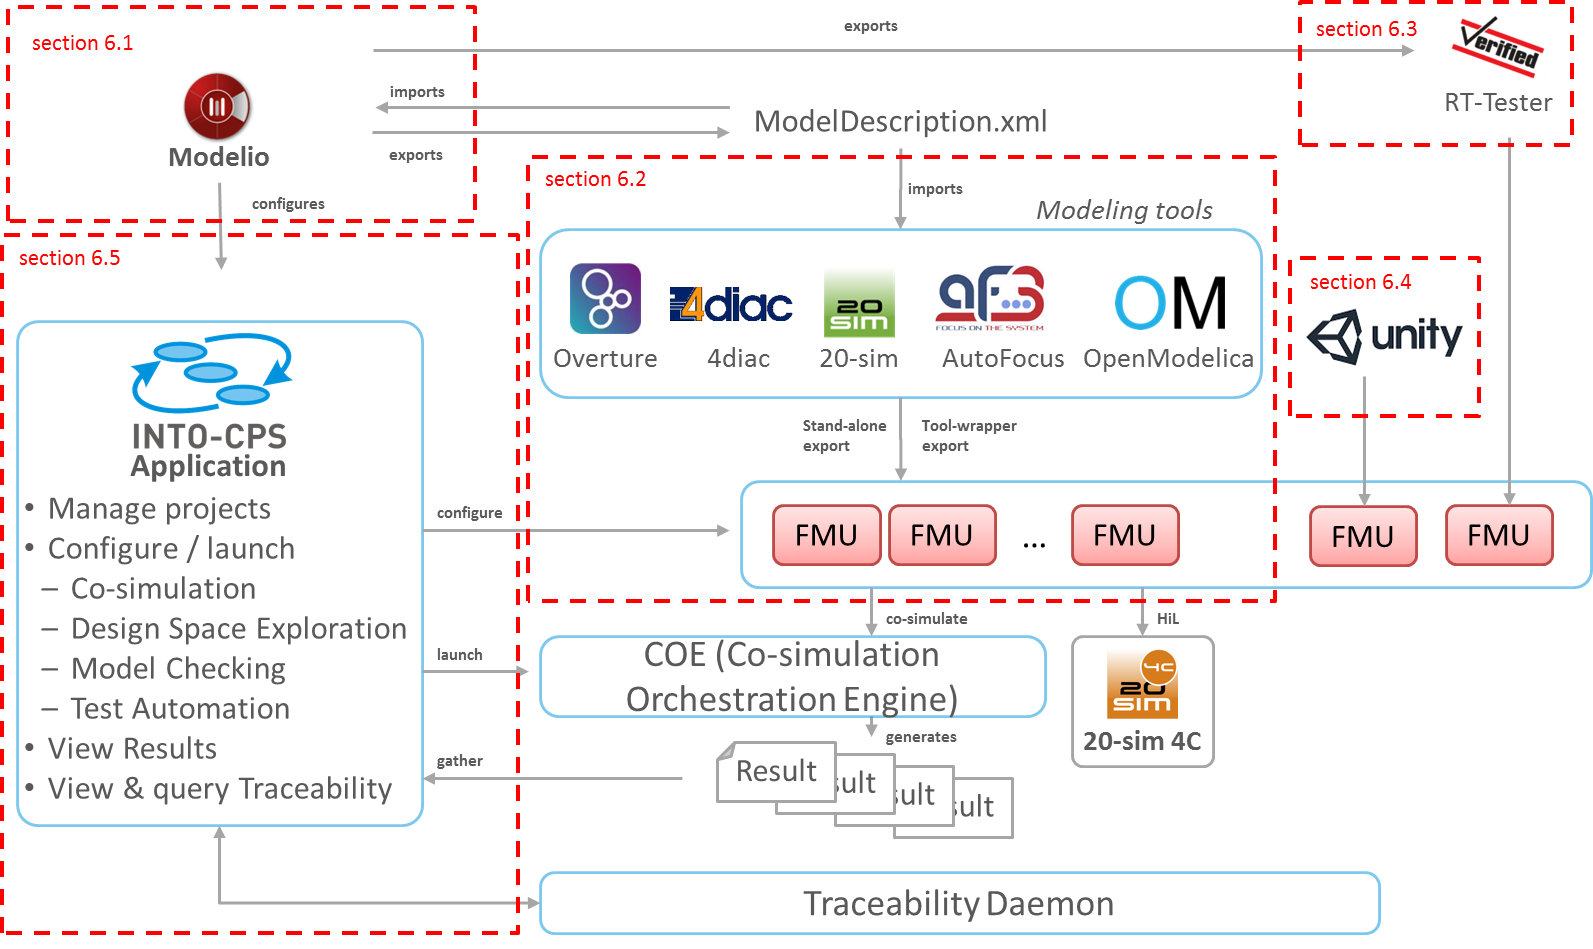
\includegraphics[width=0.9 \textwidth]{./figures/toolchain_association}
	\caption{Overview of the different tools and their arrangement in a tool-chain.}
	\label{fig:tool-chain}
\end{figure}
%[Figure of the overall tool-chain]

\subsection{Modelio}
\label{sec:modelio}
Modelio is an open-source modeling environment for various formalisms with many interfaces to import and export models. In the context of INTO-CPS, the support for SysML modelling is of primary importance, while Modelio can be extended with a range of modules to enable more modelling languages. In the terminology of the methods guidelines (e.g. \cite{INTOCPSD3.3a}), Modelio is a tool for the \textit{architectural modeling} and for \textit{requirements management}.

During the INTO-CPS project, a SysML profile was created, which is currently available as a module for Modelio 3.4 and 3.6 (see \url{http://forge.modelio.org/projects/intocps}). This INTO-CPS SysML profile extends Modelio with several functionalities that described in detail elsewhere (refs). Here, only those parts of the INTO-CPS SysML profile are discussed that add features for interconnectivity in the tool-chain.

To support the FMI multi-modelling approach, ModelDescription.xml files can now be imported into, and exported from a SysML Architectural Modeling diagram. Importing ModelDescription.xml files creates a SysML block with the corresponding flow ports and attributes, exporting them allows import in other modeling tools, such as those described below.

The Connections Diagram describes the signal flow between the different SysML blocks, which can each correspond to one FMU. Using the new INTO-CPS SysML profile, the Connections Diagram can be exported to an intermediary JSON format, which can then be imported by the INTO-CPS Application, to create a new Multi-Model.

%The INTO-CPS SysML Profile\\
%Import of ModelDescription.xml \\
%Export of ModelDescription.xml files (for modeling tools)\\
%Export of Connections Diagram (for the Application)\\

Diagrams for handling of Design Space Exploration (DSE) were created for Modelio, also included in the INTO-CPS SysML profile. These diagrams allow connection of parameters with singals, definition of objectives for a DSE, connection of signals with objectives, and ranking of results. Using these diagrams, a complete DSE configuration can be exported from Modelio.

Behavioural models that are designed in Modelio as state machines can be exported as \texttt{.xmi} files, so that they can be imported to the RT Tester tools

%DSE modeling configuration\\
Requirements management\\
Traceability\\

\subsection{Modeling tools}

Most modelling tools support the same functions. A ModelDescription.xml file (e.g. one that is automatically created from Modelio, see previous section) can be imported to create a skeleton model with the input and output signals and exposed parameters. After the actual modeling work is done, the model can be exported as Functional Mock-up Unit (FMU), in accordance with the FMI 2.0 for Co-Simulation standard. This FMU can either contain all the necessary models and solvers, so that is a self-contained model (also called stand alone), or it contains libraries which call a simulation tool to execute the simulation. The latter case is called a tool wrapper FMU. Furthermore, the different steps of importing, saving and exporting generate traces which are sent to the traceability engine of the INTO-CPS Application. The following table summarizes the status of the different tools at the time of writing of this document.

\begin{table*}[ht]
	\centering
		\begin{tabular}{l|p{2.5cm}|p{2.5cm}|p{2.5cm}|p{2.5cm}}
			Tool & MD.xml import & FMU export (stand alone) & FMU export (tool wrapper) & Traceability\\
			\hline
			20-sim & yes & no & yes & yes\\
			OpenModelica & yes & yes & no & yes\\
			Overture & yes & yes & no & yes\\
			4diac & N.A. & N.A. & N.A. & N.A \\
			AutoFocus 3 & N.A. & N.A. & N.A. \\
			Cossim & N.A. & N.A. & N.A. \\
			ABS & N.A. & N.A. & N.A. \\
		\end{tabular}
	\caption{Functionalities of the modeling tools}
	\label{tab:FunctionalitiesOfTheModelingTools}
\end{table*}

\subsection{RT Tester}

Import of xsd files from Modelio\\
FMU export of test oracles \\

\subsection{3D animation}

The 3D animation FMU allows visualisation of the simulation. It is based on the Unity engine (see \url{https://unity3d.com}), and extends it by exporting the scenario and the 3D rendering as a FMU \cite{Foldager&17}. The Modelio SysML profile (see Section \ref{sec:modelio}) takes the visualisation FMU into account. The 3D animation FMU also supports Virtual Reality (VR) headsets. It has been used in multiple case studies of INTO-CPS [ref].

\subsection{The INTO-CPS Application}

The INTO-CPS Application is the central tool to integrate the different tools and artifacts, to configure and run simulations, manage results, and more. It allows configuration and execution of DSE scenarios (which can be imported from Modelio), and is a front-end for Model-checking and Test automation, by using the RT Tester tool. Furthermore, traceability data can be viewed in the Application, either in an expert view, using the Neo4J visualisation, or by pre-configured queries.

%Integration of the different artifacts\\ 
%configuration and execution of Co-Simulation\\
%Front-end for Test-automation and model checking\\
%Viewer for traceability\\
